\begin{table}
\caption{\label{tab:locProbEffect}Reliability of the IPA algorithm in terms of the location probability and overlap of the interference threshold contours for three different scenarios. }

\vspace{0mm}
\begin{tabular}{cccc}
\hline
          	&                 & $\Delta$ &	contour				\\
          	&                 & ($\%$)	& overlap ($\%$) PU	\\\hline
 example 1	& update 1				&	7				&	0							\\
 (2000 nodes)&update 2      	&	7				&	0							\\
            & update 3       	&	7.1			& 0							\\\hline 
 example 2	& update 1      	&	8				& 0							\\ 
 (1500 nodes)& update 2				& 9.1			& 0.3						\\\hline
            & update 1 				& 7.9			&	0							\\	
 example 2	& update 2 				& 7.9			&	0							\\	
 (1800 nodes)& update 3 			& 7.9			&	0							\\	
	          & update 4 				& 10.6			&	0							\\\hline		            

\end{tabular}
\vspace{-5mm}
\end{table}

\begin{figure}
\centering
\subfloat[primary transmitter]{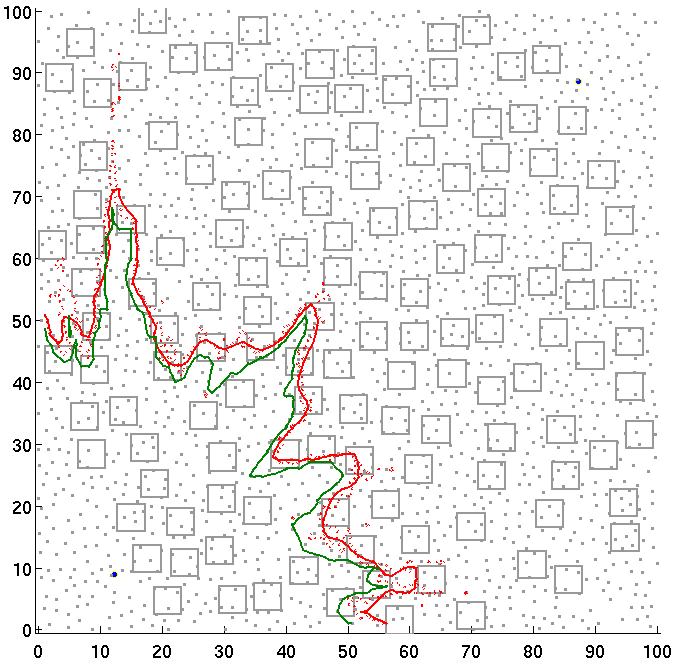
\includegraphics[scale=0.18]{figures/contribution1/vb2it0}} 
\subfloat[update 1]{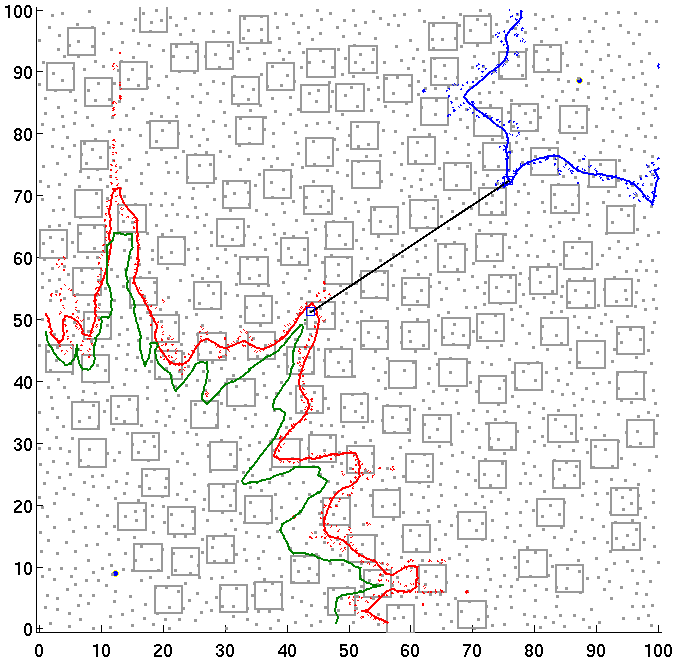
\includegraphics[scale=0.18]{figures/contribution1/vb2it1}} \\
\subfloat[update 2]{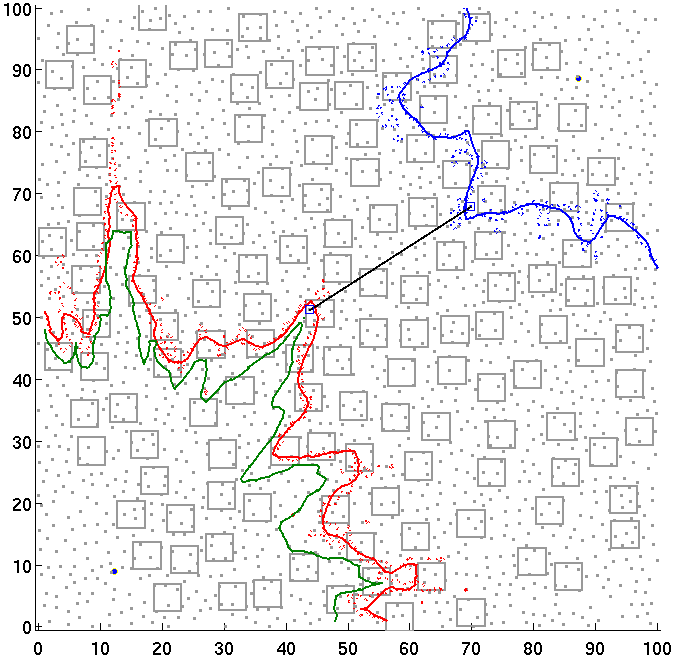
\includegraphics[scale=0.18]{figures/contribution1/vb2it2}}
\subfloat[update 3]{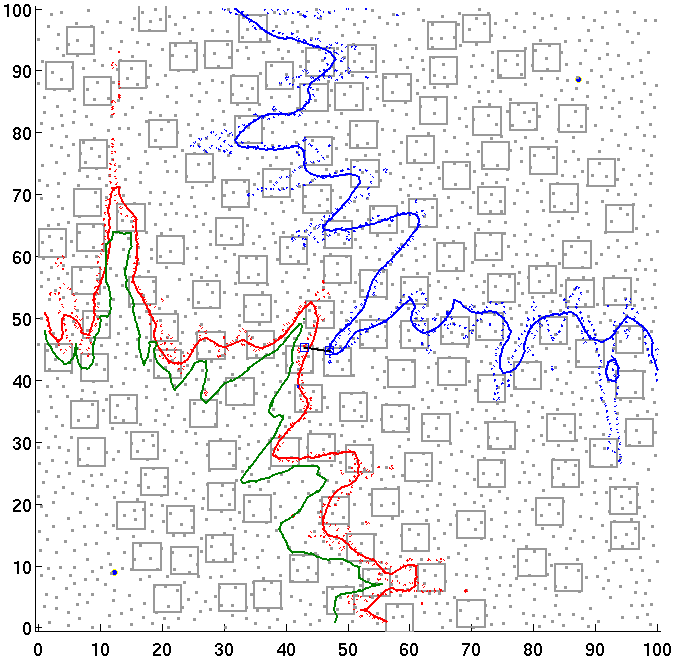
\includegraphics[scale=0.18]{figures/contribution1/vb2it3}}
\caption{\label{fig:iterationsLP} Demonstration of the IPA algorithm for example 2 from 
Tab.~\ref{tab:locProbEffect}. A primary transmitter is present in the lower left corner of the scenario and its interference threshold contour is indicated in red. The $95\%$ location probability contour is indicated in green. In the upper right corner a secondary transmitter is present with the interference contour indicated in blue.}
\end{figure}